\section{Project Area}
The Project Area is defined in order to manage in the best way the resources for the Project's lifecycle. All the Business process in this area aim to satisfy a part of the ``productive chain'' related to the Software environment and illustrated by the Software Engeenering discipline. The major aim of the area is to regroup each activity directly correlated with the Project to simplify the working procedure.

In this area there are several responsible, above all there is the Analyst who lead the practical Project develop, but parallel there is the Project Manager that need to achieve the better planning of the resources to improve the general efficiency. The charge may be covered by the same person. Other interesting roles are that which appear in the Working team organization unit illustrated on figure \ref{2img:working}; there may be several working team composed by upon two or more people and that works in a specific facet of the project.


\subsection{Requirement analysis}

\begin{figure}[ht!]
\begin{centering}
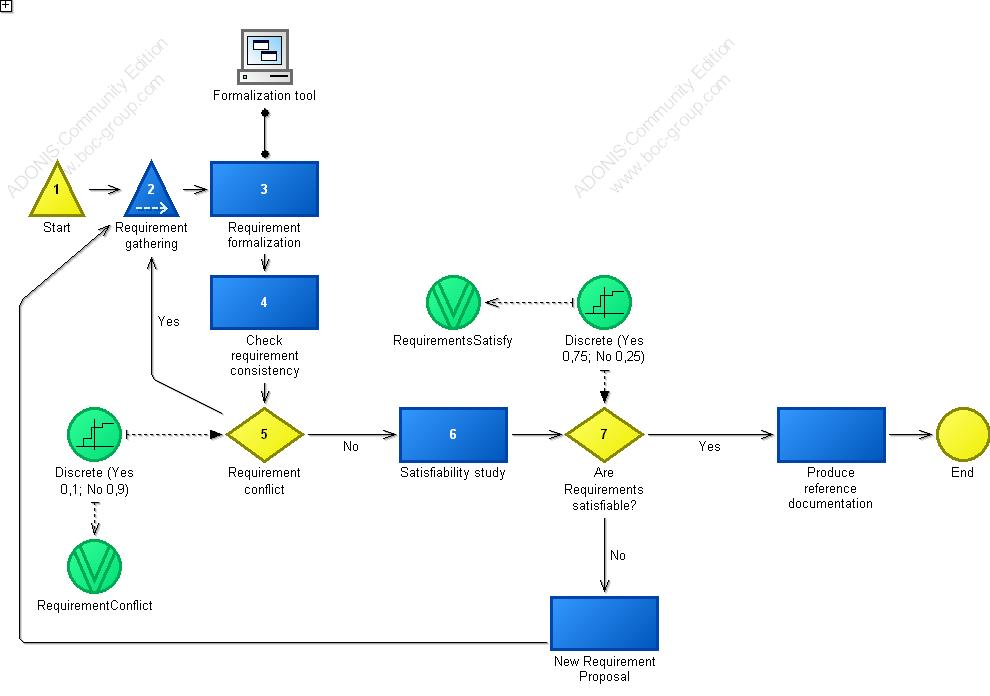
\includegraphics[scale=0.50, angle=90]{assign2/adonis/imgs/requirement.jpg}
\caption{AllSpark Requirement analysis.}
\label{2img:requirement}
\end{centering}
\end{figure}


\subsubsection{Path Analysis}

\begin{alltt}

\end{alltt}


\subsubsection{Capacity Analysis}


\begin{landscape}
\begin{table}
\centering
{\tiny
\begin{tabular}{|l|l|l|l|l|l|l|}
Business process&Activity&Performer&Number&Execution time&Cycle time&Costs\\
\hline

\end{tabular}
}
\caption{Capacity analysis for Requirement analysis.}
\end{table}
\end{landscape}
%

%

\subsection{Desing/Planning project}

\begin{figure}[ht!]
\begin{centering}
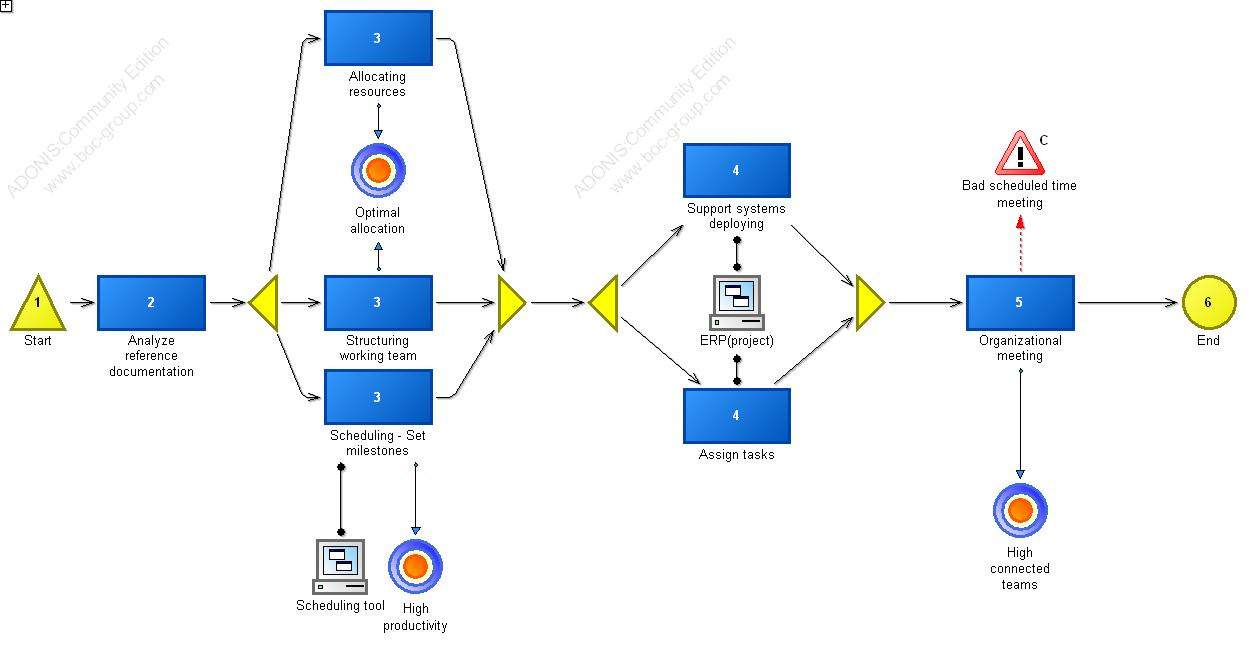
\includegraphics[scale=0.50, angle=90]{assign2/adonis/imgs/design.jpg}
\caption{AllSpark Design/Planning project.}
\label{2img:desing}
\end{centering}
\end{figure}


\subsubsection{Path Analysis}

\begin{alltt}

\end{alltt}


\subsubsection{Capacity Analysis}


\begin{landscape}
\begin{table}
\centering
{\tiny
\begin{tabular}{|l|l|l|l|l|l|l|}
Business process&Activity&Performer&Number&Execution time&Cycle time&Costs\\
\hline

\end{tabular}
}
\caption{Capacity analysis for Design/Planning project.}
\end{table}
\end{landscape}
%

%

\subsection{Implementation}

\begin{figure}[ht!]
\begin{centering}
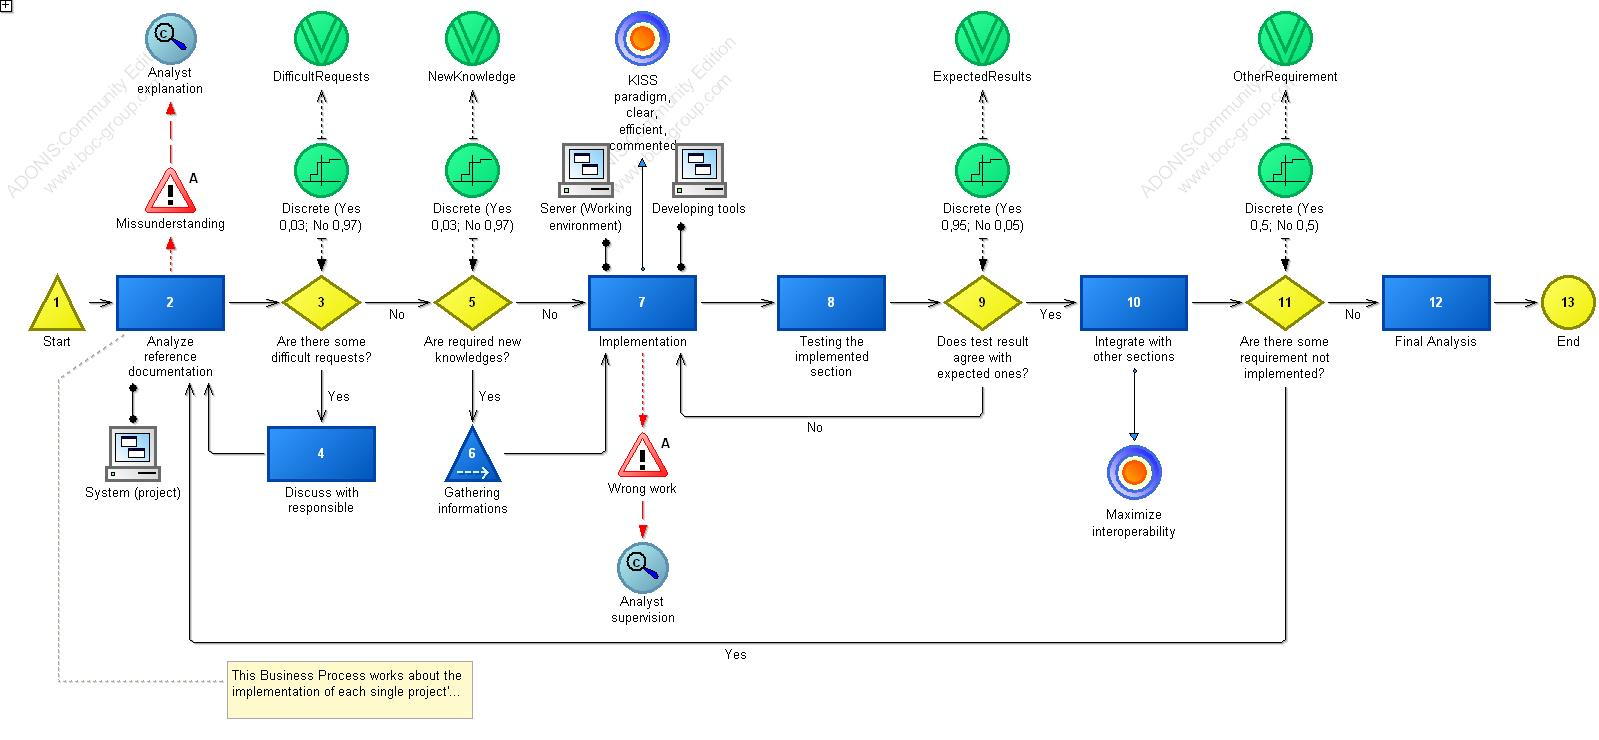
\includegraphics[scale=0.30, angle=90]{assign2/adonis/imgs/implementation.jpg}
\caption{AllSpark Implementation.}
\label{2img:implementation}
\end{centering}
\end{figure}


\subsubsection{Path Analysis}

\begin{alltt}

\end{alltt}


\subsubsection{Capacity Analysis}


\begin{landscape}
\begin{table}
\centering
{\tiny
\begin{tabular}{|l|l|l|l|l|l|l|}
Business process&Activity&Performer&Number&Execution time&Cycle time&Costs\\
\hline

\end{tabular}
}
\caption{Capacity analysis for Implementation.}
\end{table}
\end{landscape}
%

%

\subsection{Project Deployment}

\begin{figure}[ht!]
\begin{centering}
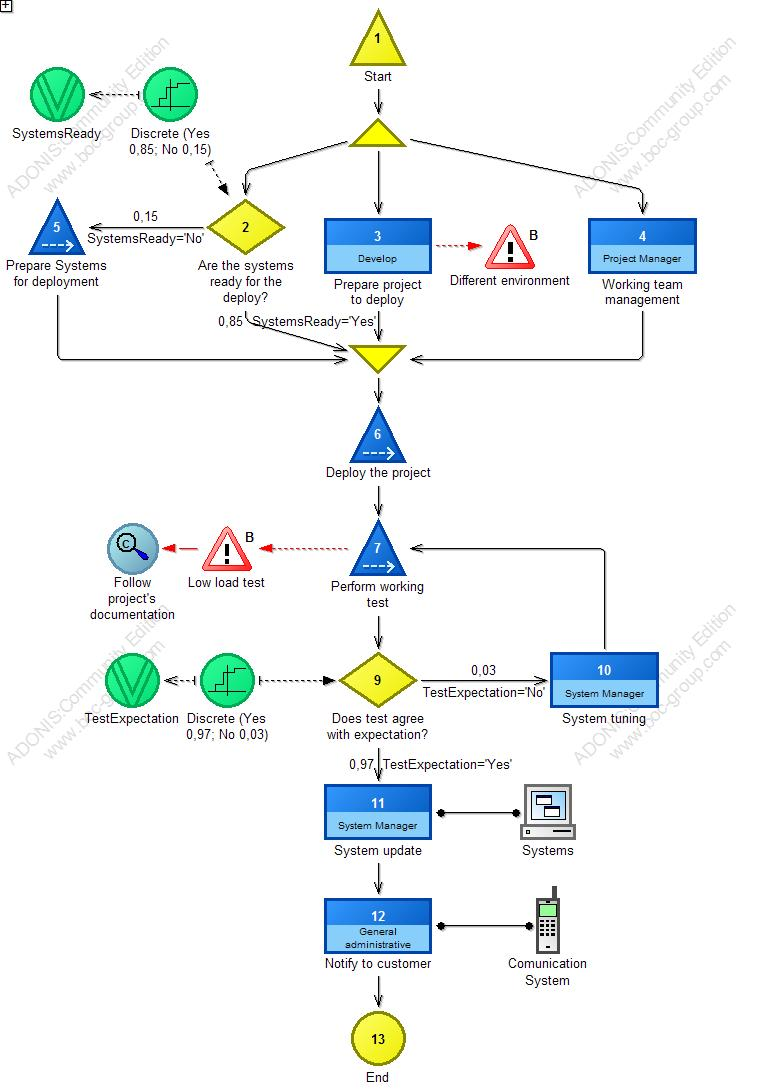
\includegraphics[scale=0.50]{assign2/adonis/imgs/deploy.jpg}
\caption{AllSpark Project Deployment.}
\label{2img:deploy}
\end{centering}
\end{figure}


\subsubsection{Path Analysis}

\begin{alltt}

\end{alltt}


\subsubsection{Capacity Analysis}


\begin{landscape}
\begin{table}
\centering
{\tiny
\begin{tabular}{|l|l|l|l|l|l|l|}
Business process&Activity&Performer&Number&Execution time&Cycle time&Costs\\
\hline

\end{tabular}
}
\caption{Capacity analysis for Deployment.}
\end{table}
\end{landscape}
%

%

\subsection{Project closure}

\begin{figure}[ht!]
\begin{centering}
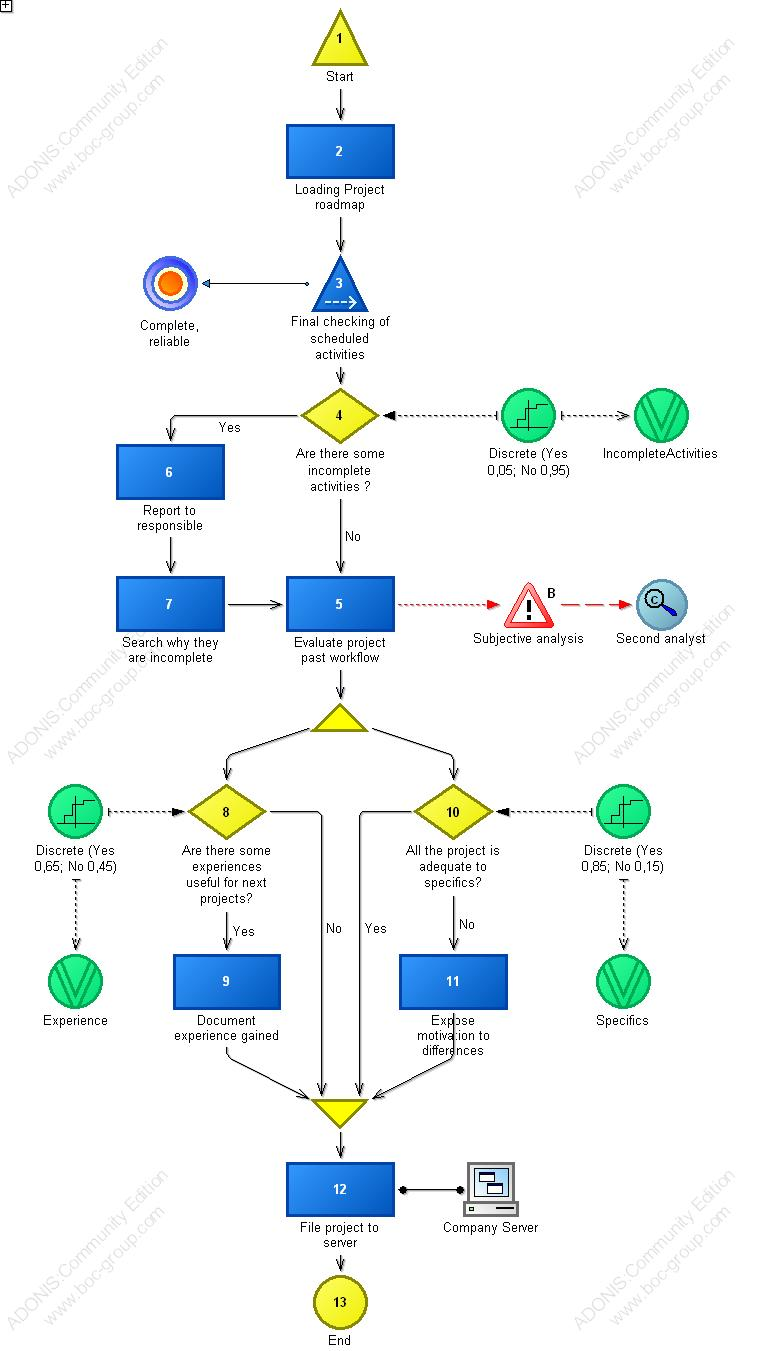
\includegraphics[scale=0.50]{assign2/adonis/imgs/closure.jpg}
\caption{AllSpark Project Closure.}
\label{2img:closure}
\end{centering}
\end{figure}


\subsubsection{Path Analysis}

\begin{alltt}

\end{alltt}


\subsubsection{Capacity Analysis}


\begin{landscape}
\begin{table}
\centering
{\tiny
\begin{tabular}{|l|l|l|l|l|l|l|}
Business process&Activity&Performer&Number&Execution time&Cycle time&Costs\\
\hline

\end{tabular}
}
\caption{Capacity analysis for Project closure.}
\end{table}
\end{landscape}
%

%